\section{Methods}

\subsection{Mechanical model}

The system under investigation is a multi-link inverted pendulum on a cart. This setup, known for its inherent instability and dynamic nature, is a cornerstone in control theory\todo{Reference needed.}. The cart, serving as the base platform for the pendulum links, is limited to linear motion along a horizontal track, simplifying the translational dynamics to one-dimensional motion along the x-axis. The cart's movement is controlled by an externally applied force $F$, which is crucial for the system's stabilization. The magnitude and direction of this force significantly impact the system's dynamics, providing a means to counteract the gravitational torque imposed by the pendulum links. 

\begin{figure}[h]
\centering
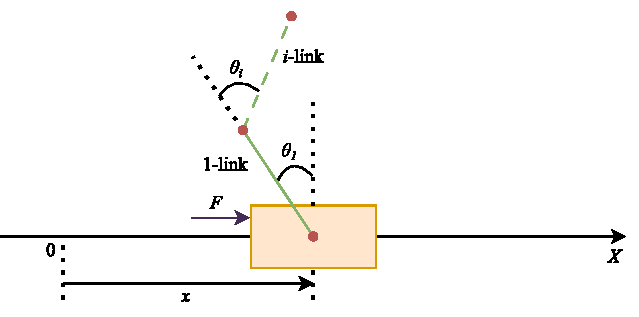
\includegraphics[width=10cm]{Figures/PendulumFinal_.pdf}
\caption{$N$-link inverted pendulum on a cart representation with link length of $1\,$m, link mass of $0.1\,$kg and cart mass of $1\,$kg~\cite{manzl2023relrl}}
\label{fig: n-pendulum on a cart}
\end{figure}

Attached to the cart is a series of n rigid links, each connected end-to-end by revolute joints. These joints allow for free rotational movement in the vertical plane, and each link 
$i$ is characterized by length $l$ and angle $\vartheta$.
This model, with its high degree of control difficulty and relevance to real-world applications, provides a valuable platform for testing sophisticated control algorithms, including those based on Reinforcement Learning.

\subsection{Reinforcement learning with continuous action space}
Reinforcement Learning (RL) is a branch of machine learning where an agent learns optimal behavior through systematic interaction with a dynamic environment, aiming to maximize cumulative rewards. This learning paradigm is distinct from supervised learning; in RL, the agent is not explicitly instructed which actions to take. Instead, it must explore and discover which actions yield the highest rewards by trial and error, a process often facilitated by a policy—a decision-making function that maps states of the environment to actions to be taken in those states~\cite{sutton_reinforcement_2018}.

In our research RL is employed to train agents to manage the dynamics of a multi-link inverted pendulum on a cart, a challenging control problem characterized by \hl{the need for precision in dynamic stability}\todo{Rewrite. It is unclear what do you mean.}. The reward function in RL plays a crucial role as it guides the learning process. For instance, a reward function can be designed to penalize the agent for excessive movement away from a target state or for using too much energy, while rewarding closer approximations of the desired state, such as maintaining the pendulum in an upright position. We use the reward function, which has shown one of the best performances from our previous study
\begin{equation}
r_2 = 1 - w_p \frac{\left|p_x\right|}{\chi_\mathrm{cart}} - (1-w_p) \frac{\sum_{j=1}^\mathrm{N} \left|\vartheta_j\right|}{\mathrm{N} \chi_{\vartheta}} \label{eq:reward2}
\end{equation}
It combines a tip position $p_x$\todo{$p_x$ should be shown in the Figure 1.} with the sum of pendulum link angles $\sum_{j=1}^{N} \left|\vartheta_j\right|$, weighted by a factor $w_p$. $\chi_\mathrm{cart}$ and $\chi_{\vartheta}$ are predefined, constant position and angle thresholds, which differ from 1-link to more link systems. $\mathrm{N}$ is the number of the links.

In RL, the choice between discrete and continuous action space might significantly affect the performance of learning algorithms. Discrete action space, used in our previous study, limits the agent’s actions to a finite set of possibilities: it either applies a negative or a positive force of the same magnitude to regulate the behavior of the system. In a continuous action space the agent is provided with an interval of the control force
\begin{equation}
F = [-f_\mathrm{cart}, +f_\mathrm{cart}]
\label{eq:force}
\end{equation}
From this interval in Eq. 2\todo{Do not use magic numbers in Latex in such way. Instead use \eqref{eq:force}} the agent is free to choose any suitable control force as an action for learning the stabilization task. Since it provides more possible actions then the discrete action space, it emerges in a faster training of an agent and achieves a more smooth and robust control task execution.  
% NOTE: 1) continue with - adding a final punchline to this section
% While simpler to implement, this can restrict the agent's ability to finely tune its responses to the environment's demands.

\subsection{Curriculum learning implementation} \label{Curriculum learning implementation}
Our approach to Curriculum Learning in the domain of MSD is rooted in the incremental introduction of complexity to the learning environment of the RL agent.\todo{Which of the types of CL introduced earlier this means?} 
%Inspired by pedagogical methods where learners progress from simple to complex tasks, we designed a curriculum that starts with the fundamental aspects of mechanical control and systematically advances to more challenging scenarios.
\todo[inline=true, color=cyan]{This whole section below must be rewritten. Firstly, we discuss that we will not mention the PD control. Physically, we are introducing the translational and rotational spring-dempers. You should add new Figure (based on the Figure 1), to show this. Next, you can write why they are there. Next, that the influence of those spring-dampers will diminish as training progress. Afterwards, you can introduce the Table below and Figure 2. Please avoid asking rethoric questions.}

We have four parameters in our CL-scheme and their roles are explained in the Table 1\todo{Again, do not use magic numbers. Replace by \\ref.}.

\begin{table}[ht]
\caption{Decay types and their descriptions}
\begin{tabular}{|c|p{5cm}|}
\hline
\textbf{Curriculum Learning Parameters} & \textbf{Description} \\ \hline
Control Values & control parameters representing spring-damper values, which influence the restriction of the system behavior\\ \hline
Decay Steps & time steps when the transition to another set of Control Values occurs\\ \hline
Decay Function & describes the law on how the Control Values will be changed\\ \hline
Decay Factor & sets the speed of Decay Function\\ \hline
\end{tabular}
\end{table}

% \begin{table}[ht]
% \caption{Decay types and their descriptions}
% \begin{tabular}{|c|p{9cm}|}
% \hline
% \textbf{Decay Types} & \textbf{Description} \\ \hline
% Linear & The linear decay provides a steady and uniform reduction in control assistance. This approach is suitable when a constant rate of challenge increase is desired, allowing the agent to adapt gradually and predictably. \\ \hline
% Quadratic & This decay function introduces a progressively increasing rate of difficulty. Initially, changes are subtle, but as the agent advances, the control assistance decreases more sharply, fostering a more rapid adaptation to complex tasks. \\ \hline
% Exponential & Exponential decay is characterized by a swift reduction in assistance at the early stages, which slows down as the agent approaches the target proficiency level. This is particularly useful when the agent is expected to make significant initial progress but may require more time to refine skills as tasks become more complex. \\ \hline
% Quintic & The quintic function represents a more aggressive approach, with a slow start followed by a rapid escalation in difficulty. This can be employed when agents are expected to spend more time mastering initial stages before facing a steep increase in task complexity. \\ \hline
% Discrete & The discrete decay function operates on a segmented or stepwise reduction in control assistance. Unlike the gradual transitions seen in other decay types, discrete decay imposes a series of abrupt changes at predetermined steps in the learning process. This approach is akin to moving through distinct learning phases, each with a fixed level of difficulty. \\ \hline
% \end{tabular}
% \end{table}

Modelled spring-damper system restriction could be described as Proportional-Derivative (PD) control scheme, which with its intuitive appeal and theoretical backing, provides a reliable means to achieve initial stability, that is crucial for the early stages of learning in complex dynamical systems~\cite{franklin2010feedback}. This phase acted as a confidence-building measure, allowing agent to familiarize himself with the basics of the system’s dynamics.
Following the establishment of basic control proficiency, the curriculum progressed to a gradual reduction of the control assistance (control values), transitioning responsibility from the control algorithm to the RL agent. This methodical change was governed by predefined decay functions that dictate the rate and pattern of PD assistance withdrawal. The choice of function was determined by the desired learning trajectory and complexity of the task at hand. The comparison of decay functions behavior, which are used in our study, is showed at the Figure~\ref{fig: decay types}.
In general, decay function could be any function, which will reduce the control values via some mathematical law. The problem is - how to select the best one for our control task? For this we have conducted an analysis of them and the results of it are described in Results section. 

\begin{figure}[htb]
\centering
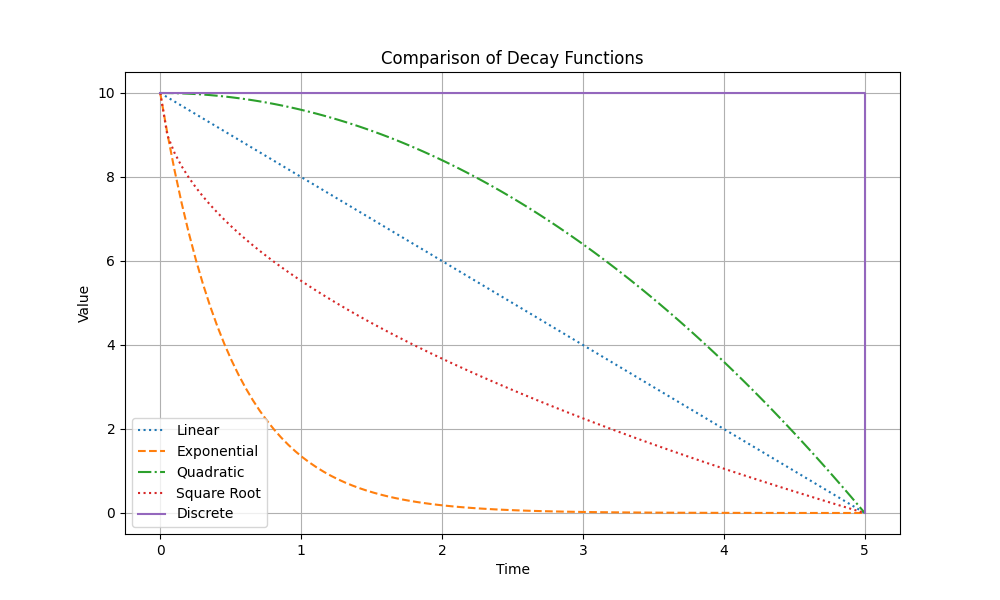
\includegraphics[width=15cm]{Figures/CL_decay_types_comparison.png}
\caption{5 decay functions comparison for a given set of control values [10, 0]. At the decay step equal to 5 all the functions take the next control value of 0.}
\label{fig: decay types}
\end{figure}

% improve that
% add a figure here, which shows the functions instead of a table. Maybe changing a table to a simple thing!!!!!!!


% \begin{table}[ht]
% \caption{Decay types and their descriptions}
% \begin{tabular}{|c|p{9cm}|}
% \hline
% \textbf{Decay Types} & \textbf{Description} \\ \hline
% Linear & The linear decay provides a steady and uniform reduction in control assistance. This approach is suitable when a constant rate of challenge increase is desired, allowing the agent to adapt gradually and predictably. \\ \hline
% Quadratic & This decay function introduces a progressively increasing rate of difficulty. Initially, changes are subtle, but as the agent advances, the control assistance decreases more sharply, fostering a more rapid adaptation to complex tasks. \\ \hline
% Exponential & Exponential decay is characterized by a swift reduction in assistance at the early stages, which slows down as the agent approaches the target proficiency level. This is particularly useful when the agent is expected to make significant initial progress but may require more time to refine skills as tasks become more complex. \\ \hline
% Quintic & The quintic function represents a more aggressive approach, with a slow start followed by a rapid escalation in difficulty. This can be employed when agents are expected to spend more time mastering initial stages before facing a steep increase in task complexity. \\ \hline
% Discrete & The discrete decay function operates on a segmented or stepwise reduction in control assistance. Unlike the gradual transitions seen in other decay types, discrete decay imposes a series of abrupt changes at predetermined steps in the learning process. This approach is akin to moving through distinct learning phases, each with a fixed level of difficulty. \\ \hline
% \end{tabular}
% \end{table}



